\documentclass[12pt]{jsarticle}
%\usepackage{geometry}                % See geometry.pdf to learn the layout options. There are lots.
%\geometry{a4paper}                   % ... or a4paper or a5paper or ... 
%\geometry{landscape}                % Activate for for rotated page geometry
%\usepackage[parfill]{parskip}    % Activate to begin paragraphs with an empty line rather than an indent
\usepackage[dvipdfmx]{graphicx}
\usepackage{amsmath, amssymb}
\usepackage{epstopdf}
\DeclareGraphicsRule{.tif}{png}{.png}{`convert #1 `dirname #1`/`basename #1 .tif`.png}

\title{古典的なノンパラメトリック検定はなにを仮定しているのか}
\author{}
%\date{}                                           % Activate to display a given date or no date

\begin{document}
\maketitle
\section{読むのがめんどうな人へ}

たぶんシミュレーションだけ見ればいい. 

\section{前置き}

もともと工学部出身のぼくが, 医学系の研究室に行っておもしろかったことはいろいろある. 

その中の一つが, 医学系の人のアーチファクト(artifact)という言葉の使い方だ. 

アーチファクトというのは, 辞書的には人工物とか工芸品を指す.

ぼくからしたら「この結果はアーチファクトだよ」とか言われたら褒められているのかな? みたいな感じがする.

でも違う. 医学系の言葉使いではアーチファクトというのは, 自然現象とか生命現象の本質じゃない人工的な混ざりもの, みたいなニュアンスだ.

ところで, ぼくは統計モデリングというのが好きだ. モデリングというのはデータを取った人からいろいろ話を聞いて, 関数とか確率分布とか微分方程式とか差分方程式とかを組み合わせて, データを取った人のイメージとか目的とかを統計の言葉に翻訳するような作業だ. モデルを作るというのは, ぼくの感覚では仮定を置くことに等しい. 

それはもうアーチファクトのかたまりみたいな作業だ.

そのせいかどうかは知らないが, 医学系の人はモデリングよりも検定が好きな印象がある. 統計屋というと, いろんな検定を知っていて, 場合に応じて正しい検定を選べる人, みたいな認識をされることもある.

なかでもノンパラメトリック検定が好きなようだ. 

ノンパラメトリック検定とは, 母集団に対して特定の確率分布を仮定しないで検定をする手法の総称とされる. 

仮定が少ないほうが客観的な分析でえらいという感覚があるんだと思う.

そこがぼくの好みと相容れない. 

でも好みじゃないのでノンパラメトリック検定に関する相談には乗りませんというのも大人げないので, これからちょっとノンパラメトリック検定について勉強していきたいと思っている.

この文書はそういったものだ. 

この文書がこれからどういったものになるかは, ぼくもまだわかってない.

でも結びの言葉はなんとなくだけど決めてある. 

「仮定を置かないんじゃなくて仮定を明確にして, アーチファクトをもってアーチファクトを制すのだ.」

\section{ノンパラメトリック・モデル}

ノンパラメトリックモデルという言葉とノンパラメトリック検定という言葉はまったく別物だと思ったほうがよさそうだ.

ノンパラメトリックモデルというのは, パラメータが多すぎるモデルのことを指す.

データのサイズにほぼ比例して, モデルのパラメータが増えるようなモデルはノンパラメトリックモデルと呼ばれる. 

以下では, ノンパラメトリックモデルの話はしない. 

ノンパラメトリック検定の話をする. 

\section{仮説検定一般に関する注意点}

仮説検定は「確率版背理法」と例えられることもあるが, 現実のデータを扱う以上, 背理法のようにすっきりとはしていない.
仮説検定では, 「帰無仮説 $H_0: \theta = 0$, 対立仮説 $H_1: \theta \neq 0$」みたいな形で「仮説」を提示する. 
しかし, 帰無仮説 $H_0$ の確率を評価するのに, 帰無分布というのを作らなくちゃいけない.

仮説検定には, 「$H_0: \theta = 0$」といった\textbf{意識されやすい仮定}と検定のやり方(何検定を使うか)を決めた時点で置かれている\textbf{意識されにくい仮定}が存在する. 例えば「○○検定を行った」と言った時点で, 「サンプルは正規分布に従う」とか「サンプルは独立同分布とする」とかの意識されにくい仮定はクリアされたことになっている. 

仮説検定を行った結果, 帰無仮説が棄却されたというと意識されやすい仮定が棄却された感じがするが, 実は意識されにくい仮定のほうがもっとずれていたのかもしれない.

「$H_0$でないから$H_1$だ」という背理法ほど, 仮説検定はすっきりしていない.

\section{符号検定(Sign Test)}

検定というのは帰無分布を一つ決めて, そこからのずれを測っている. 

帰無分布を決めなきゃいけないのに, 「特定の確率分布を仮定しない」なんてことができるのか. 

どうやらできるようだ.

データ $X_1, X_2, \ldots, X_n$ を生成した分布が連続な分布関数 $F$ を持つということだけを仮定しよう. これはどちらかというと意識されにくい仮定だ.$\theta$ を $F$ の中央値とする. 

その上で母集団の中央値が0であるという帰無仮説を検定したい. 
まず, 帰無仮説 $H_0: \theta = 0$, 対立仮説 $H_1: \theta > 0$ の片側検定を考える.

そして, 
\begin{align}
S_n = \sum_{i=1}^{n} I_{\{X_i > 0\}}
\end{align}
という統計量を作ることにする. ここで $I_A$ は指示関数(つまり $X_i > 0$ なら 1, さもなくば 0 を返す)である. 

$S_n$ は符号が + になった回数を単に数えただけだ. 

帰無仮説のもとで, $S_n$ は二項分布 $\mathrm{Binomial}(n, 1/2)$ に従う.

中央値(メジアン)の定義を確認しておくと, 分布 $F$ に従う確率変数を $X$ と書くとき, 
\begin{align}
\Pr(X \ge m) \ge \frac{1}{2}, \quad \Pr(X \ge m) \ge \frac{1}{2}
\end{align}
を満たす実数 $m$ が中央値である. 

分布関数が連続であれば, 
\begin{align}
\Pr(X \le m) = \frac{1}{2}
\end{align}
である. 
いま, $X$ が連続な分布関数を持つことを仮定したので, 帰無分布が二項分布 $\mathrm{Binomial}(n, 1/2)$ になるのは, ほぼ定義そのものである.

帰無仮説のもとで $A$ という事象の起こる確率を $\Pr_{H_0}(A)$ と書くことにすると, この検定の有意水準 $\alpha$ での棄却域は, $\Pr_{H_0}(S_n>k)\le\alpha$ を満たす $k$に対して$S_n>k$ となる範囲である.

対立仮説 $H_1: \theta < 0$ の片側検定をやりたい場合, 棄却域は, $\Pr_{H_0}(S_n<k)\le\alpha$ を満たす $k$に対して$S_n>k$ となる範囲である.

対立仮説 $H_1: \theta \neq 0$ の両側検定をやりたい場合, 棄却域は, $\Pr_{H_0}(\min(S_n,n-S_n)<k)\le\alpha/2\}$ を満たす $k$に対して$S_n<k$ となる範囲である.

中央値が0である場合だけでなく, 一般の $\theta_0$ の検定を考えたいときは, $X_i$ それぞれから $\theta_0$ を引いてやれば, 同じ問題に帰着される. 

2群の比較ならわかるけど, 1群の検定なんて使う場面あるのかと思うかもしれないので, こんな例を与えておく:「患者さんたちにある睡眠薬を飲ませたところ, 睡眠時間がそれぞれ増えたり減ったりしました. 睡眠時間の増減の中央値が0より大きけば, 睡眠薬は効果ありと言えそうです.」

\paragraph{0がある場合.} 
連続型の分布を仮定したので, 理想的にはちょうど0が出る確率は0である.
現実的には0がある場合はそれをのぞいて検定統計量を出す.

\subsection{Rによる実装例}

統計ソフト R で上記の符号検定のp値を計算するには, 次のように書けばよい.
まず, 対立仮説 $H_1: \theta > 0$ の片側検定の場合,
\begin{verbatim}
theta0 <- 0
n <- length(X)
Sn <- sum(X>theta0)
pbinom(Sn-1,n,0.5,lower.tail = FALSE)
\end{verbatim}
対立仮説 $H_1: \theta > 0$ の片側検定の場合, 
\begin{verbatim}
pbinom(Sn-1,n,0.5,lower.tail = FALSE)
\end{verbatim}
対立仮説 $H_1: \neq  0$ の両側検定の場合, 
\begin{verbatim}
2*pbinom(min(Sn,n-Sn),n,0.5)
\end{verbatim}
こう書いても同じ.
\begin{verbatim}
2*min(pbinom(Sn-1,n,0.5,lower.tail = FALSE),pbinom(Sn,n,0.5))
\end{verbatim}

\section{Wilcoxon の符号付き順位検定(Wilcoxon Signed-Rank Test)}
符号検定は符号の情報しか使っていないので, 検出力はあまり高くないことが予想される. (本当にそうなのかは, \ref{simu1sample}節で検討する予定)

そこで, データの順位の情報も使うことを考える. 

$R_i$ を $X_i$ の順位とする.
フォーマルに書くと,
\begin{align}
R_i = \#\{j;X_j\le X_i\}
\end{align}
である. ここで, $\#A$ は集合 $A$ の 要素の個数を返す関数である.

次の統計量を考える.
\begin{align}
T = \sum_{i=1}^{n}R_i I_{\{X_i>0\}}
\end{align}
ここで分布 $F$ の密度関数が0を中心に左右対称であるという仮定をする. 「0を中心に」というのは意識されやすい仮定, 「左右対称である」というのは意識されにくい仮定だ.
この仮定のもとで, $ I_{\{X_i>0\}}$ はベルヌーイ分布 $\mathrm{Bernoulli}(1/2)$ に従う.

$\{R_i, I_{\{X_i>0\}}\}$は$n$個の順位それぞれと, 0か1なので, 取りうる組み合わせは$2^n$通りある. 
その中で $T=k$ となる場合の数の合計を $c_{n,k}$ とすると, $\Pr\{T=k\} = c_{n,k}/2^n$ と書ける. これが帰無分布である.

データから求めた $T$ の実現値を $T_0$ とするとき, 
\begin{itemize}
\item 帰無仮説 $H_0: \theta = 0$, 対立仮説 $H_1: \theta > 0$ の片側検定の p 値は $\Pr\{T \ge T_0\}$, 
\item 帰無仮説 $H_0: \theta = 0$, 対立仮説 $H_1: \theta < 0$ の片側検定の p 値は $\Pr\{T \le T_0\}$,
\item 帰無仮説 $H_0: \theta = 0$, 対立仮説 $H_1: \neq  0$ の両側検定の p 値は
$T > n(n+1)/4$ のとき, $\Pr\{T \ge T_0\}$, さもなくば $\Pr\{T \le T_0\}$
\end{itemize}
となる.
ここで $n(n+1)/4$ というのは, $T$の取りうる値の範囲 0 から $\sum_{i=1}^{n} i= n(n+1)/2$ のまんなかである.

中央値が0である場合だけでなく, 一般の $\theta_0$ の検定を考えたいときは, $X_i$ それぞれから $\theta_0$ を引いてやれば, 同じ問題に帰着される.

\subsection{シミュレーション}
\label{simu1sample}

よい検定の第1条件はまずなによりも実際の $\alpha$ エラーが, 設定した有意水準以下であることだ. 
これが成り立っていないとオオカミ少年になってしまい, どんなに検出力が高くても評価されない. 

なのでここではまず $\alpha$ エラーのシミュレーションを行う.

正規分布でやるとノンパラメトリック検定のありがたみがわからないので, まずはロジスティック分布 $\mathrm{Logistic}(0,1)$ からサンプリングしたデータで, 帰無仮説 $H_0: \theta = 0$, 対立仮説 $H_1: \neq  0$ の両側検定を行い p 値の分布を調べる. 

ロジスティック分布は正規分布と似た形をしており, 左右対称だが正規分布より裾が重い.

サンプルサイズ $n=5$ のときのシミュレーション結果を, 図\ref{fig_pv_logis_5_t}-\ref{fig_pv_logis_5_wilco}に示す.

これらの図では横軸にシミュレーションした$\alpha$ エラー, 縦軸に名目上の有意水準を取ってプロットした. 
折れ線(実線)が対角線より下に来ていれば, $\alpha$ エラーが名目上の有意水がより下に保たれていることを示す.

\begin{figure}[htbp]
  \begin{center}
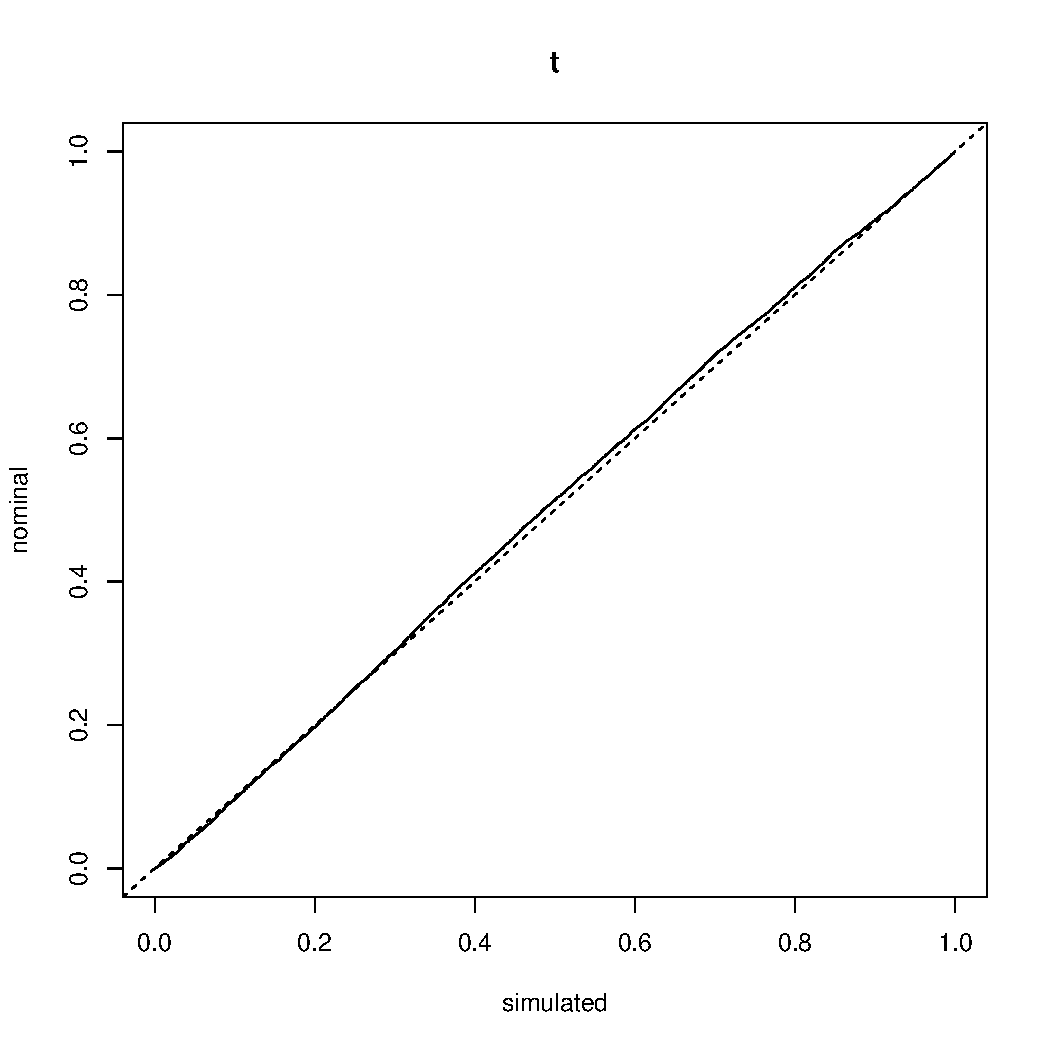
\includegraphics[width=70mm]{img/pv_logis_5_t.pdf}
  \end{center}
     \caption{$\alpha$ エラーのプロット. ロジスティック分布 $\mathrm{Logistic}(0,1)$. $n=5$. t 検定}
  \label{fig_pv_logis_5_t}
 \end{figure}
 
 \begin{figure}[htbp]
 \begin{center}
  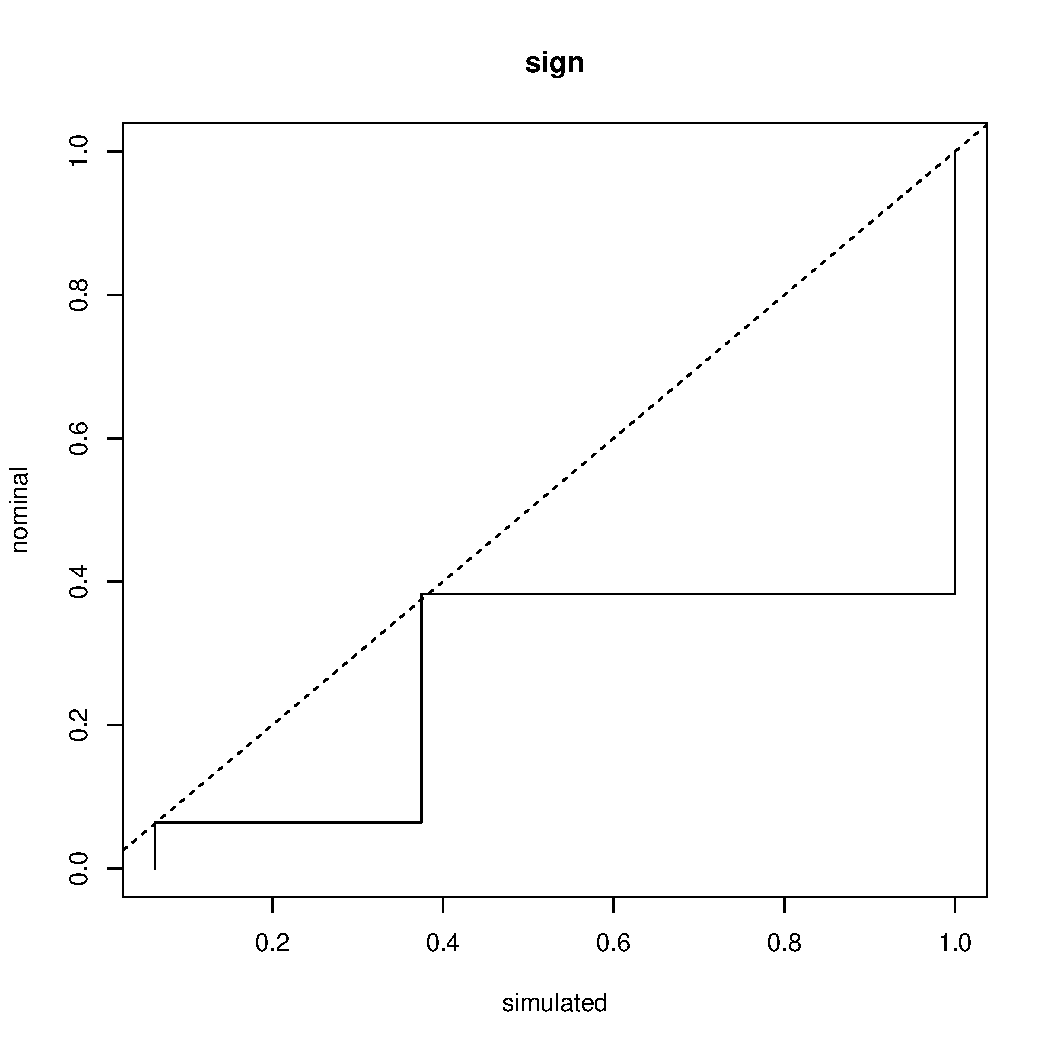
\includegraphics[width=70mm]{img/pv_logis_5_sign.pdf}
 \end{center}
      \caption{$\alpha$ エラーのプロット. ロジスティック分布 $\mathrm{Logistic}(0,1)$. $n=5$. 符号検定.}
     \end{figure}  

 \begin{figure}[htbp]
 \begin{center}
  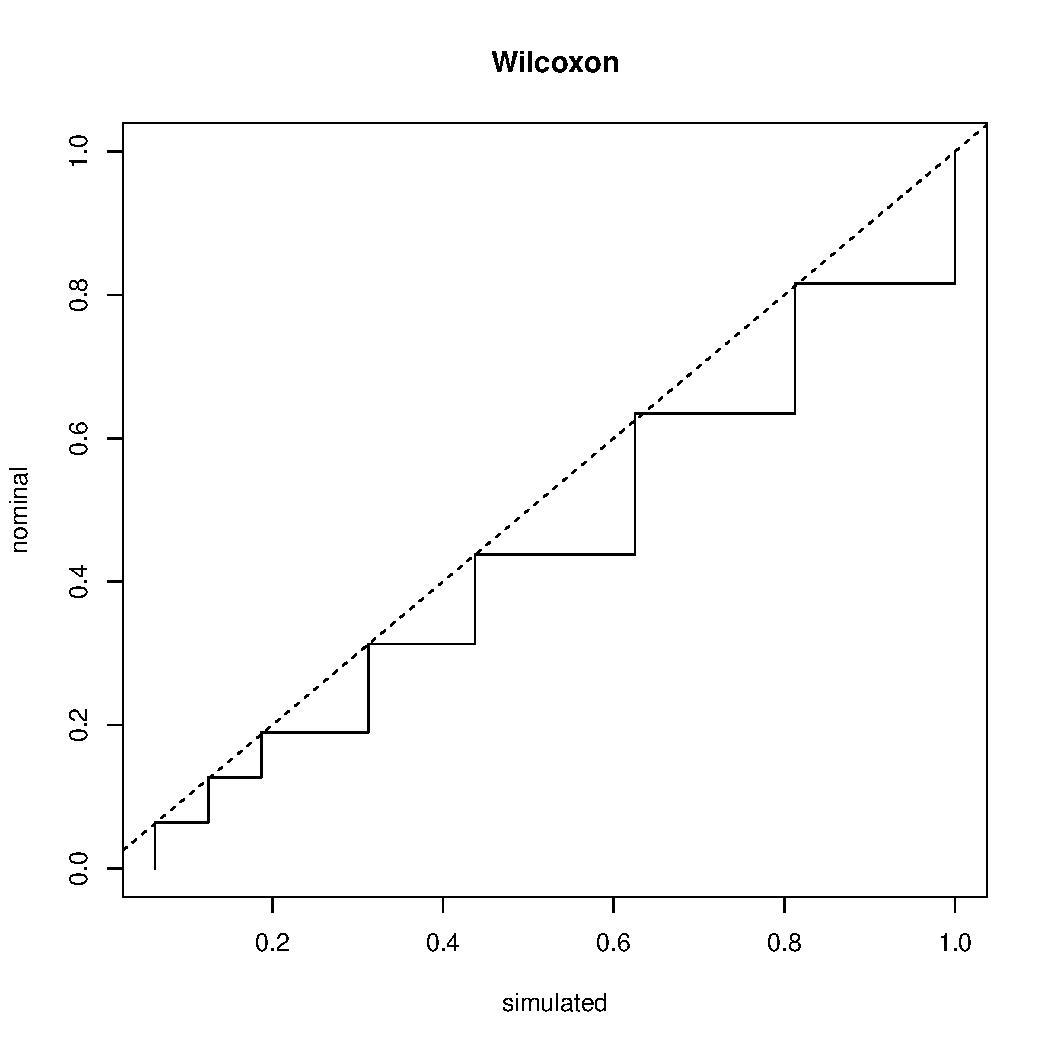
\includegraphics[width=70mm]{img/pv_logis_5_wilco.pdf}
 \end{center}
       \caption{$\alpha$ エラーのプロット. ロジスティック分布 $\mathrm{Logistic}(0,1)$. $n=5$. Wilcoxon の符号付き順位検定.}
  \label{fig_pv_logis_5_wilco}
\end{figure}

$t$ 検定はサンプルサイズが小さくても, 割と名目通りの p 値を与えている. 

ノンパラメトリック検定は離散的な p 値を与える. 特に符号検定でその傾向が顕著である.

正規分布に似た形だと t 検定も使えそうなので, 一様分布 $\mathrm{Uniform}(-1,1)$ で同様の検定をやってみよう(図\ref{fig_pv_unif_5_t}-\ref{fig_pv_unif_5_wilco}).

\begin{figure}[htbp]
  \begin{center}
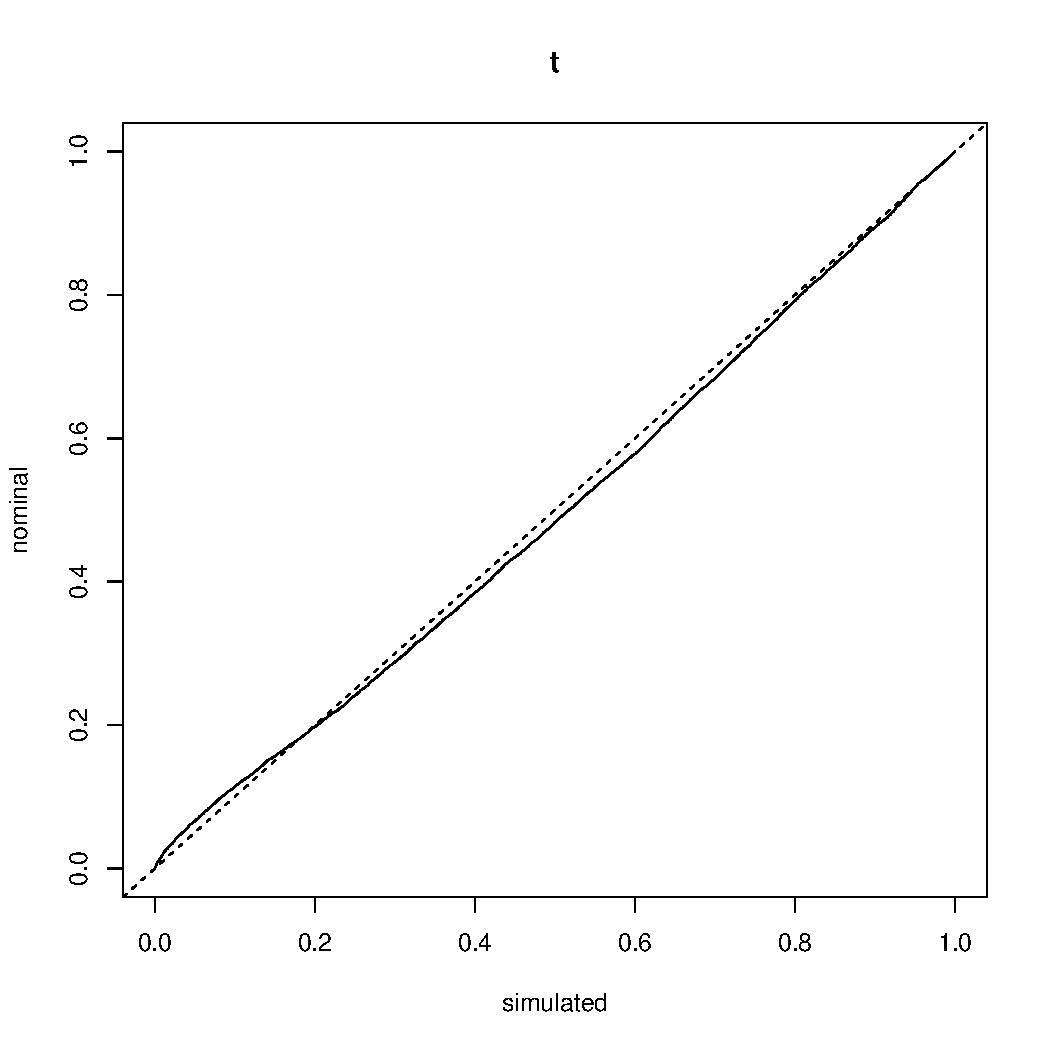
\includegraphics[width=70mm]{img/pv_unif_5_t.pdf}
  \end{center}
     \caption{$\alpha$ エラーのプロット. 一様分布 $\mathrm{Uniform}(0,1)$. $n=5$. t 検定}
  \label{fig_pv_unif_5_t}
 \end{figure}
 
 \begin{figure}[htbp]
 \begin{center}
  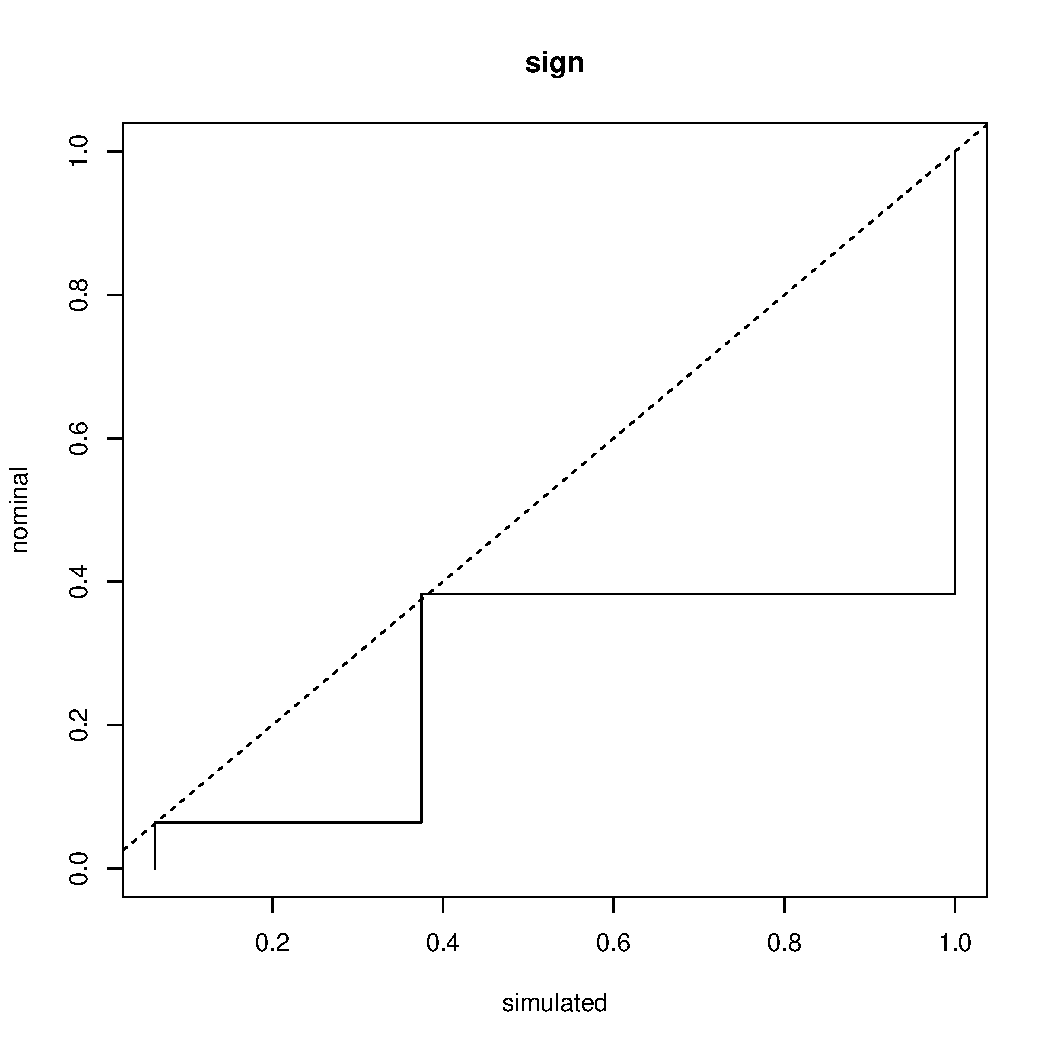
\includegraphics[width=70mm]{img/pv_unif_5_sign.pdf}
 \end{center}
      \caption{$\alpha$ エラーのプロット. 一様分布 $\mathrm{Uniform}(0,1)$. $n=5$. 符号検定.}
     \end{figure}  

 \begin{figure}[htbp]
 \begin{center}
  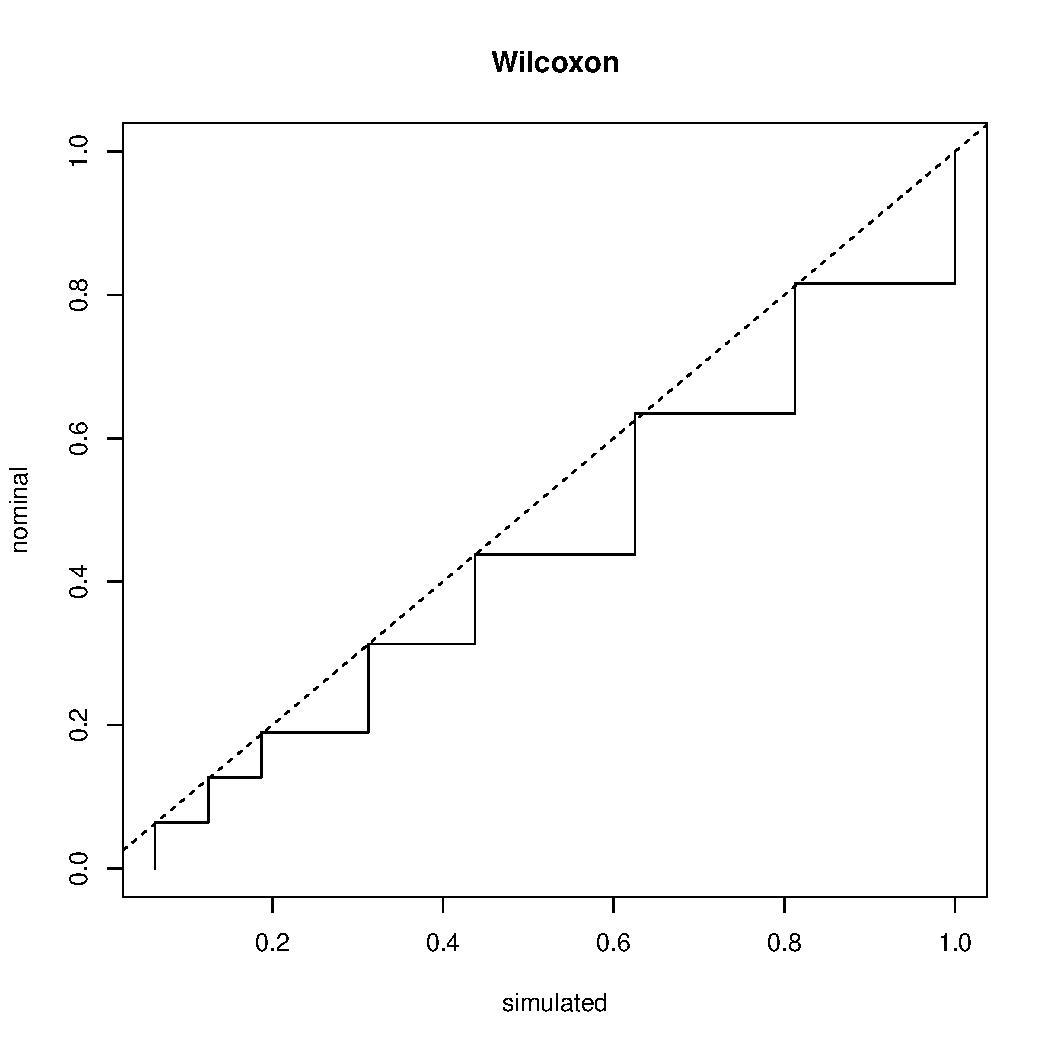
\includegraphics[width=70mm]{img/pv_unif_5_wilco.pdf}
 \end{center}
       \caption{$\alpha$ エラーのプロット. 一様分布 $\mathrm{Uniform}(0,1)$. $n=5$. Wilcoxon の符号付き順位検定.}
  \label{fig_pv_unif_5_wilco}
\end{figure}

$t$ 検定は有意水準が小さいときに少しだけ, $\alpha$ エラーが有意水準を上回っている.

サンプルサイズを10まで増やすと(図\ref{fig_pv_unif_10_t}-\ref{fig_pv_unif_10_wilco}), t 検定でもかなり正確な p 値を与える.

\begin{figure}[htbp]
  \begin{center}
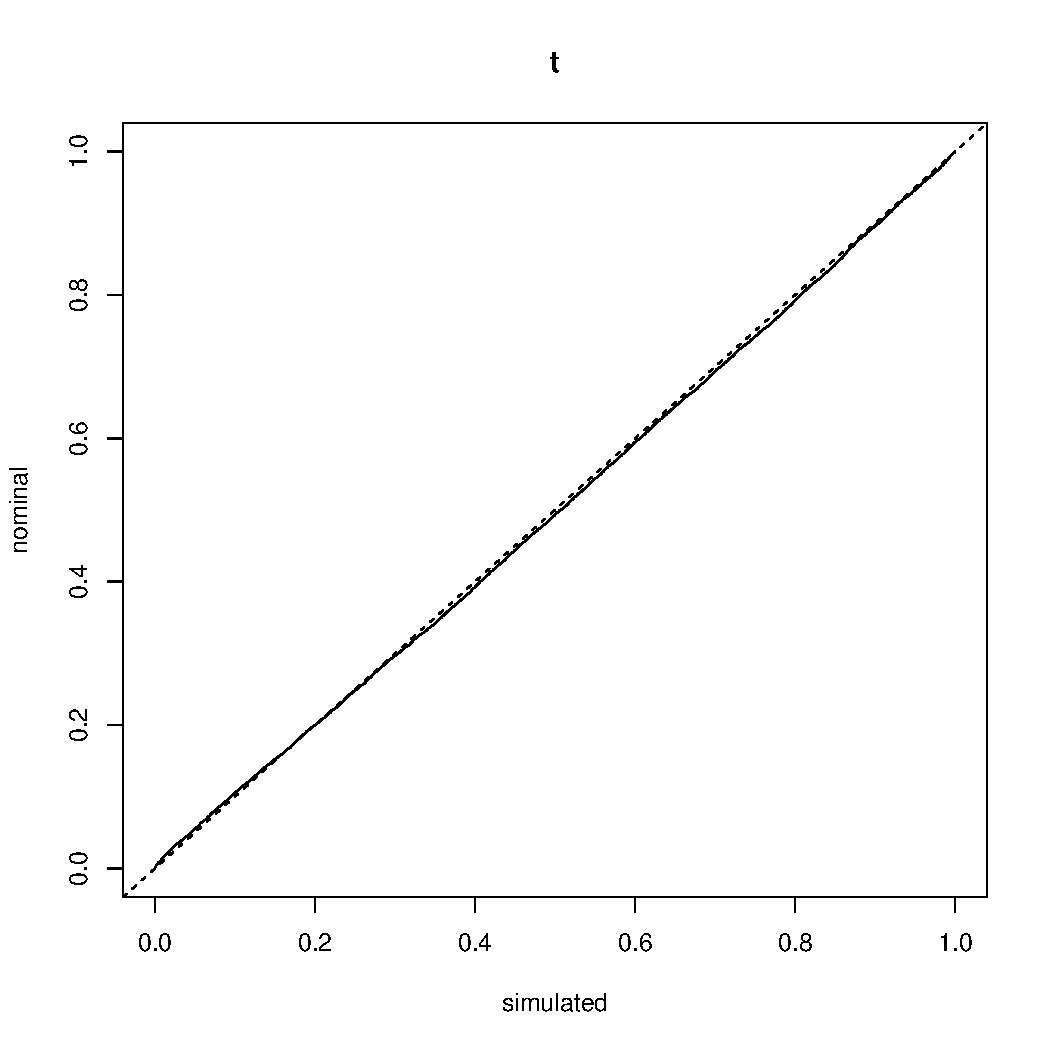
\includegraphics[width=70mm]{img/pv_unif_10_t.pdf}
  \end{center}
     \caption{$\alpha$ エラーのプロット. 一様分布 $\mathrm{Uniform}(0,1)$. $n=10$. t 検定}
  \label{fig_pv_unif_10_t}
 \end{figure}
 
 \begin{figure}[htbp]
 \begin{center}
  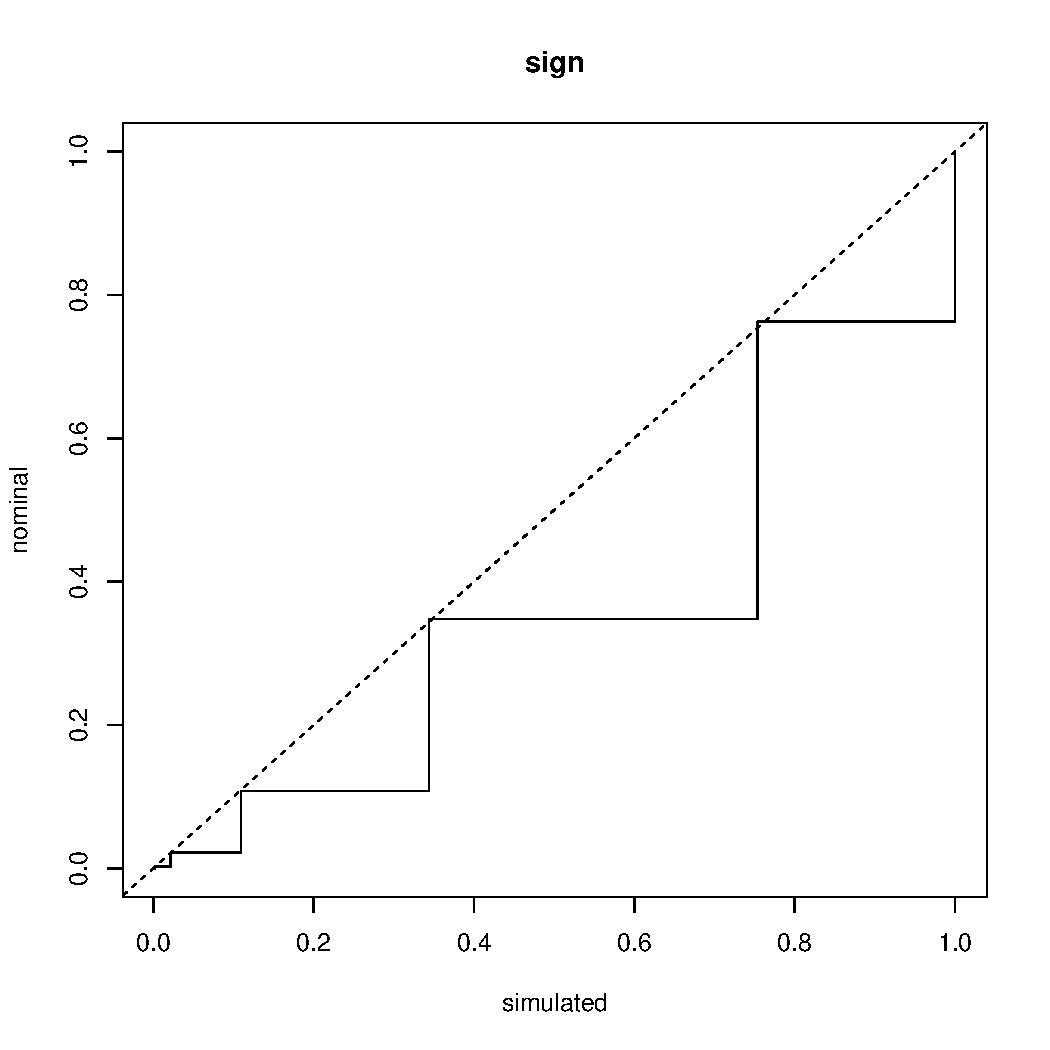
\includegraphics[width=70mm]{img/pv_unif_10_sign.pdf}
 \end{center}
      \caption{$\alpha$ エラーのプロット. 一様分布 $\mathrm{Uniform}(0,1)$. $n=10$. 符号検定.}
     \end{figure}  

 \begin{figure}[htbp]
 \begin{center}
  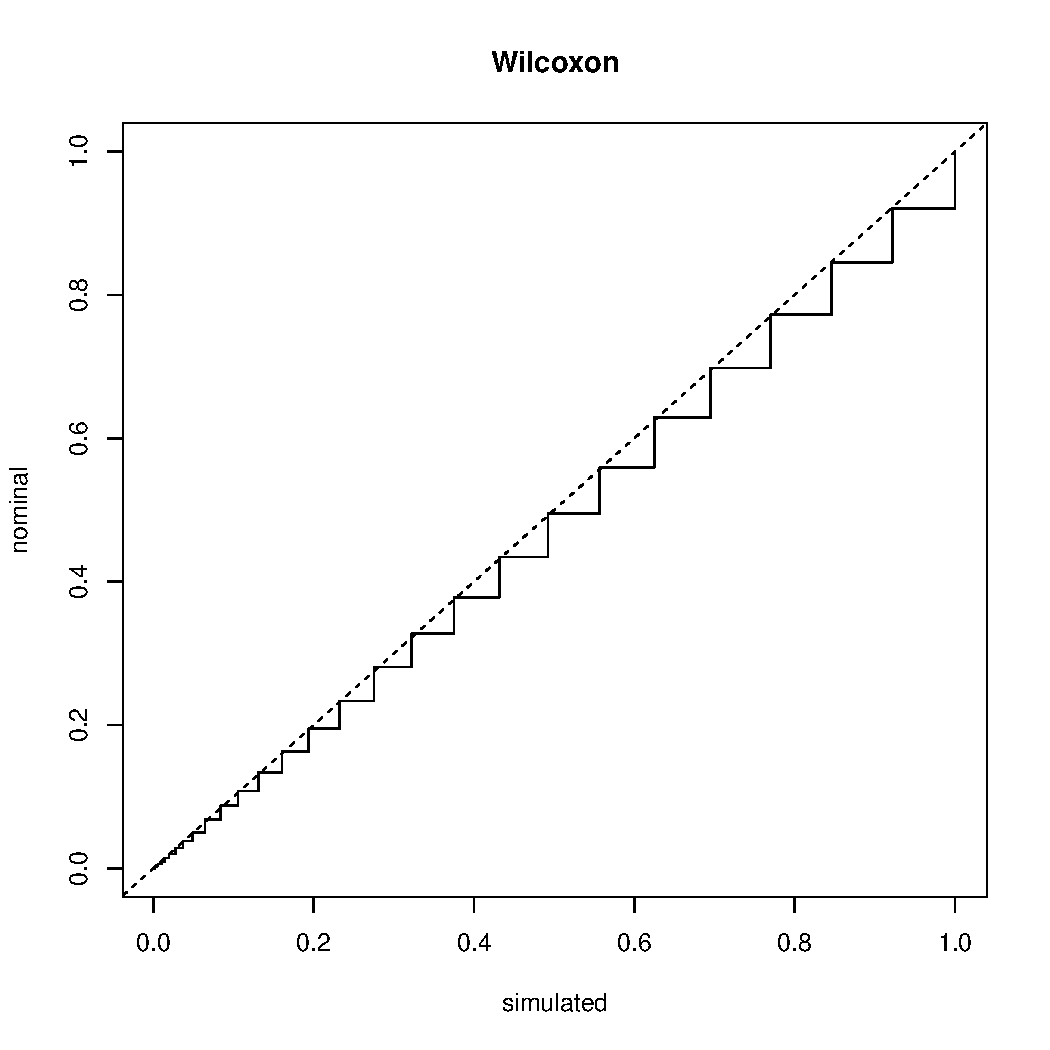
\includegraphics[width=70mm]{img/pv_unif_10_wilco.pdf}
 \end{center}
       \caption{$\alpha$ エラーのプロット. 一様分布 $\mathrm{Uniform}(0,1)$. $n=10$. Wilcoxon の符号付き順位検定.}
  \label{fig_pv_unif_10_wilco}
\end{figure}

次は, 左右対称の仮定を崩してみる. 

ワイブル分布 $\mathrm{Weibull}(m ,\eta)$ は $m>1$ のとき, モードの周りにやや集中した形をとり, $m < 1$ のとき, 指数分布よりも裾の重い分布となる. 
ワイブル分布は左右対称でないので, t 検定では平均 $\mu$に対しての, 帰無仮説 $H_0: \mu = \mu_0$, 対立仮説 $H_1: \mu \neq \mu_0$, 符号検定とWilcoxon の符号付き順位検定では中央値 $\theta$ に関しての, 帰無仮説 $H_0: \theta = \theta_0$, 対立仮説 $H_1: \theta \neq \theta_0$ の検定を行った. 

まず, $\mathrm{Weibull}(2 ,1)$ からサンプリングして $n=5$のときを図\ref{fig_pv_weibull_2_1_5_t}-\ref{fig_pv_weibull_2_1_5_wilco} に示す.

\begin{figure}[htbp]
  \begin{center}
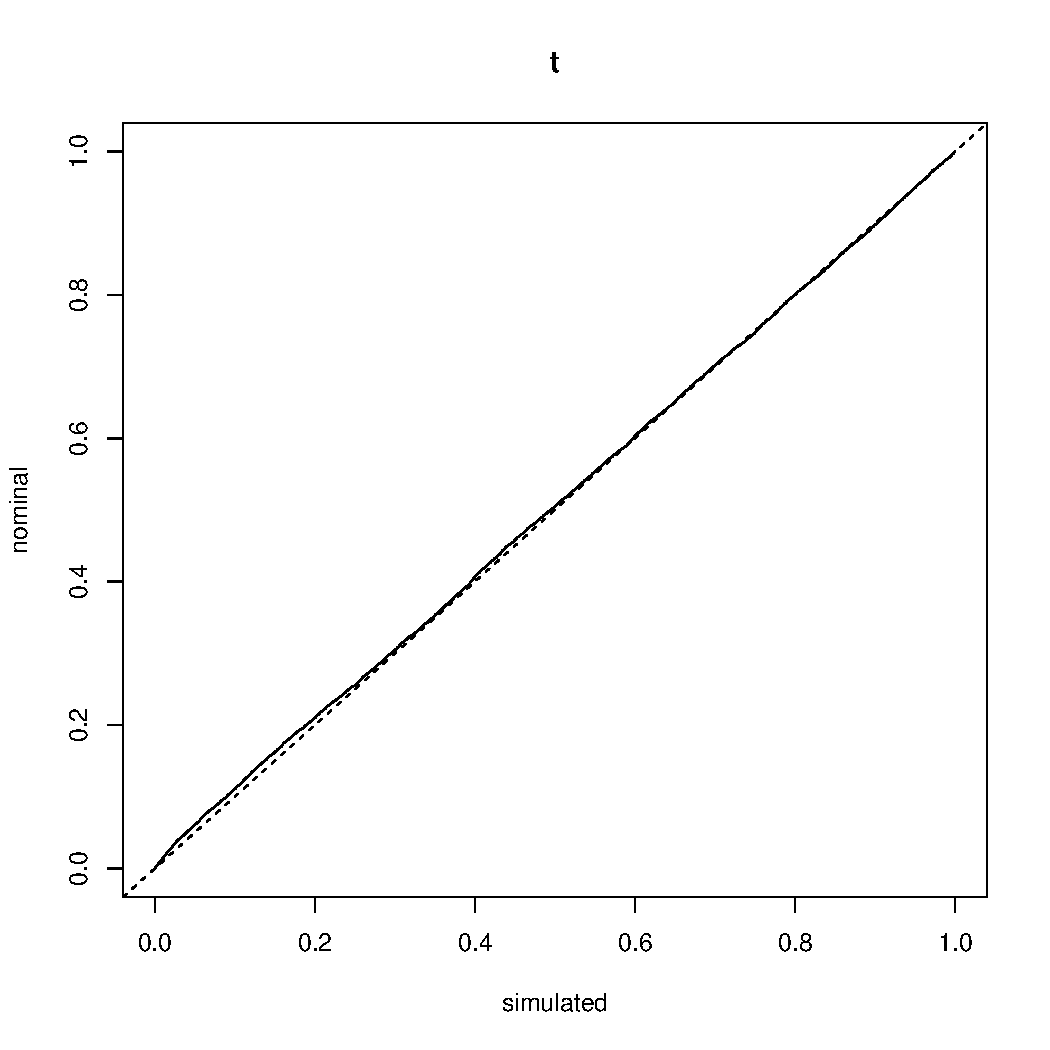
\includegraphics[width=70mm]{img/pv_weibull_2_1_n5_t.pdf}
  \end{center}
     \caption{$\alpha$ エラーのプロット. ワイブル分布 $\mathrm{Weibull}(2,1)$. $n=5$. t 検定}
  \label{fig_pv_weibull_2_1_5_t}
 \end{figure}
 
 \begin{figure}[htbp]
 \begin{center}
  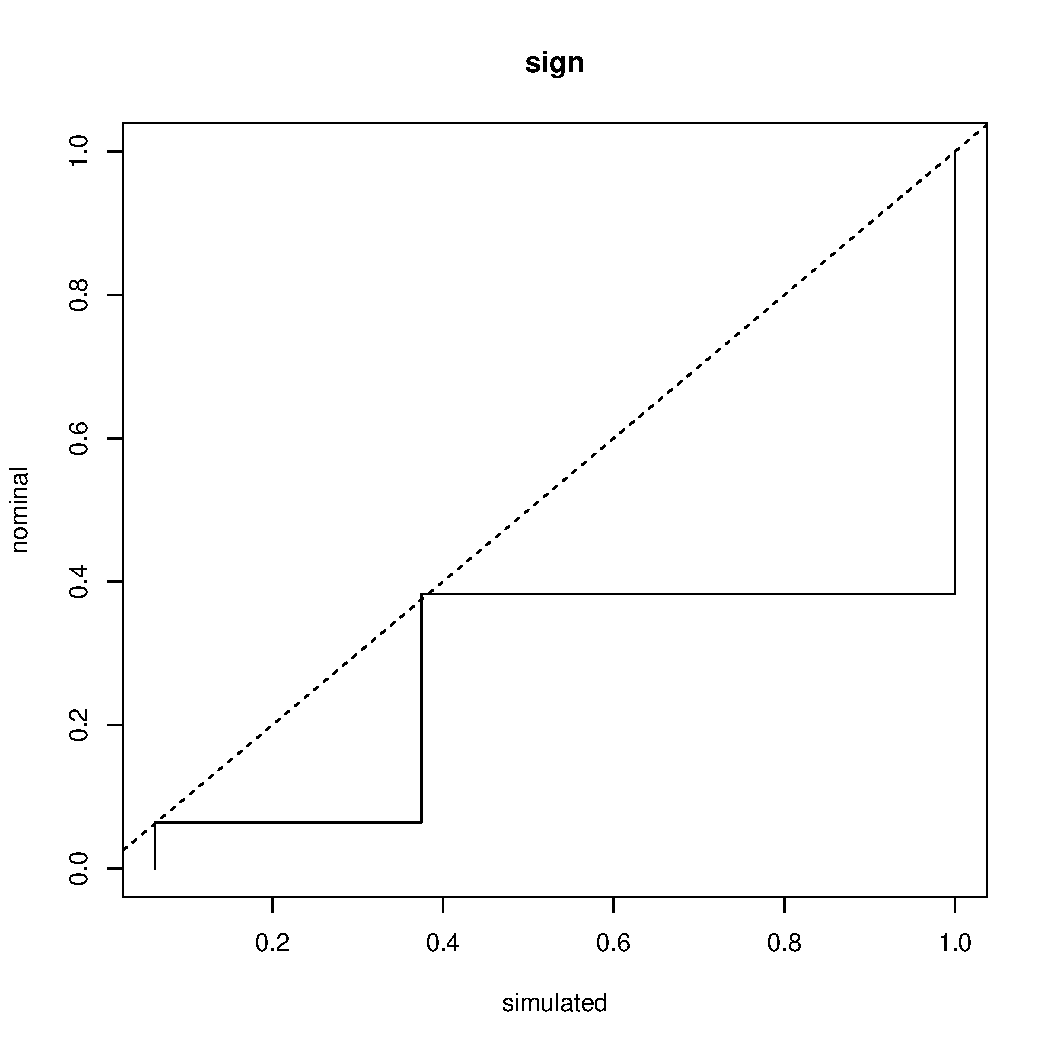
\includegraphics[width=70mm]{img/pv_weibull_2_1_n5_sign.pdf}
 \end{center}
      \caption{$\alpha$ エラーのプロット. ワイブル分布 $\mathrm{Weibull}(2,1)$. $n=5$. 符号検定.}
     \end{figure}  

 \begin{figure}[htbp]
 \begin{center}
  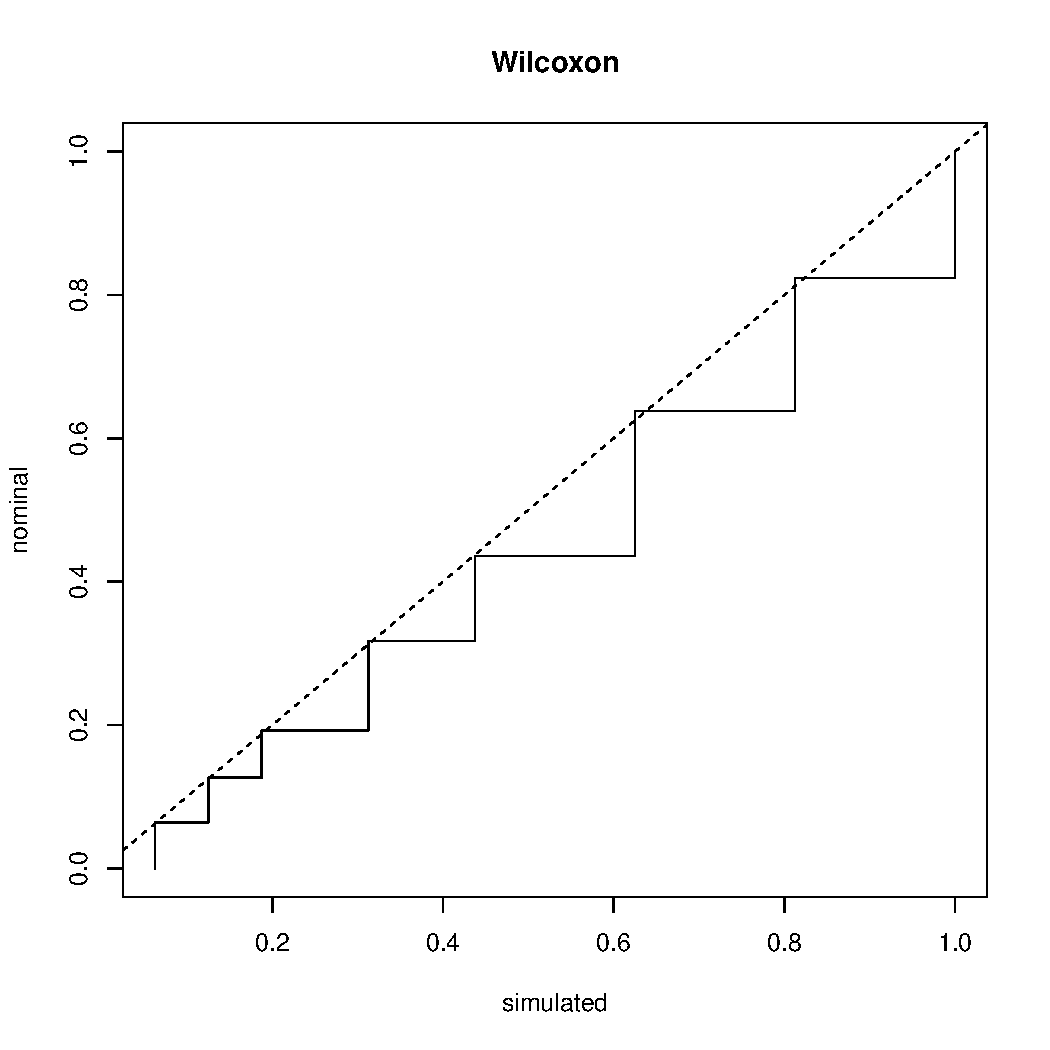
\includegraphics[width=70mm]{img/pv_weibull_2_1_n5_wilco.pdf}
 \end{center}
       \caption{$\alpha$ エラーのプロット. ワイブル分布 $\mathrm{Weibull}(2,1)$. $n=5$. Wilcoxon の符号付き順位検定.}
  \label{fig_pv_weibull_2_1_5_wilco}
\end{figure}

Wilcoxon の符号付き順位検定, もっと崩れるかと思ったけど意外といい.

次に $\mathrm{Weibull}(0.5 ,1)$ からサンプリングして $n=5$のときを図\ref{fig_pv_weibull_05_1_5_t}-\ref{fig_pv_weibull_05_1_5_wilco} に示す.

\begin{figure}[htbp]
  \begin{center}
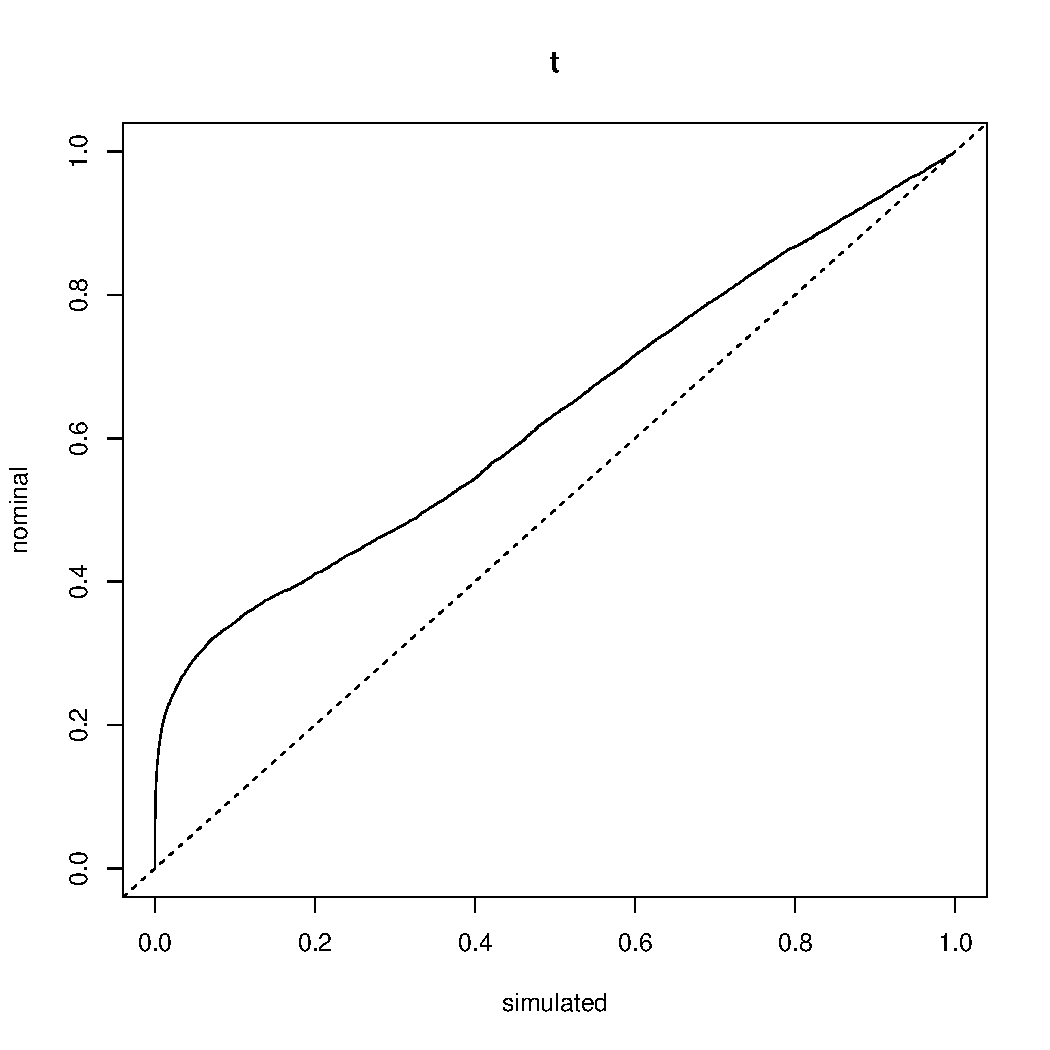
\includegraphics[width=70mm]{img/pv_weibull_05_1_n5_t.pdf}
  \end{center}
     \caption{$\alpha$ エラーのプロット. ワイブル分布 $\mathrm{Weibull}(0.5,1)$. $n=5$. t 検定}
  \label{fig_pv_weibull_05_1_5_t}
 \end{figure}
 
 \begin{figure}[htbp]
 \begin{center}
  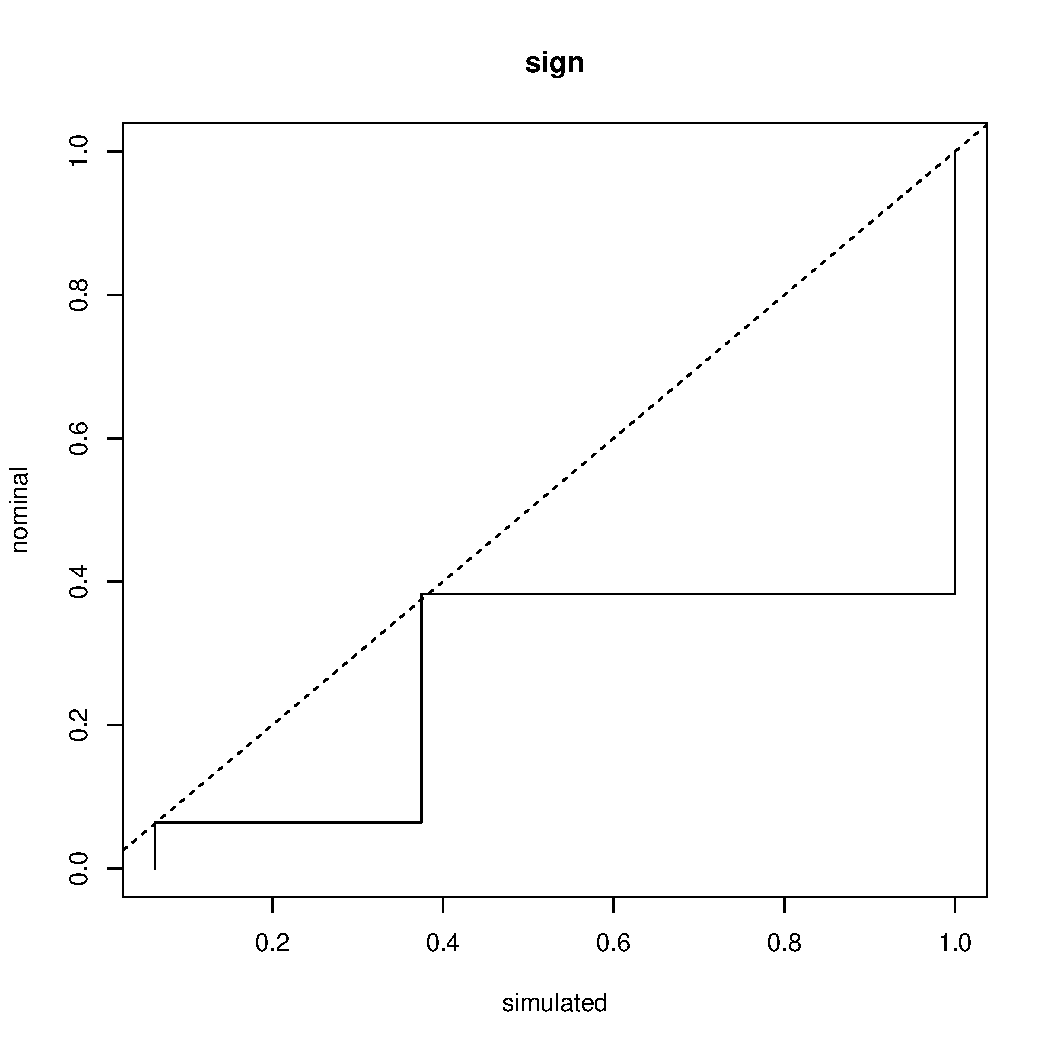
\includegraphics[width=70mm]{img/pv_weibull_05_1_n5_sign.pdf}
 \end{center}
      \caption{$\alpha$ エラーのプロット. ワイブル分布 $\mathrm{Weibull}(0.5,1)$. $n=5$. 符号検定.}
     \end{figure}  

 \begin{figure}[htbp]
 \begin{center}
  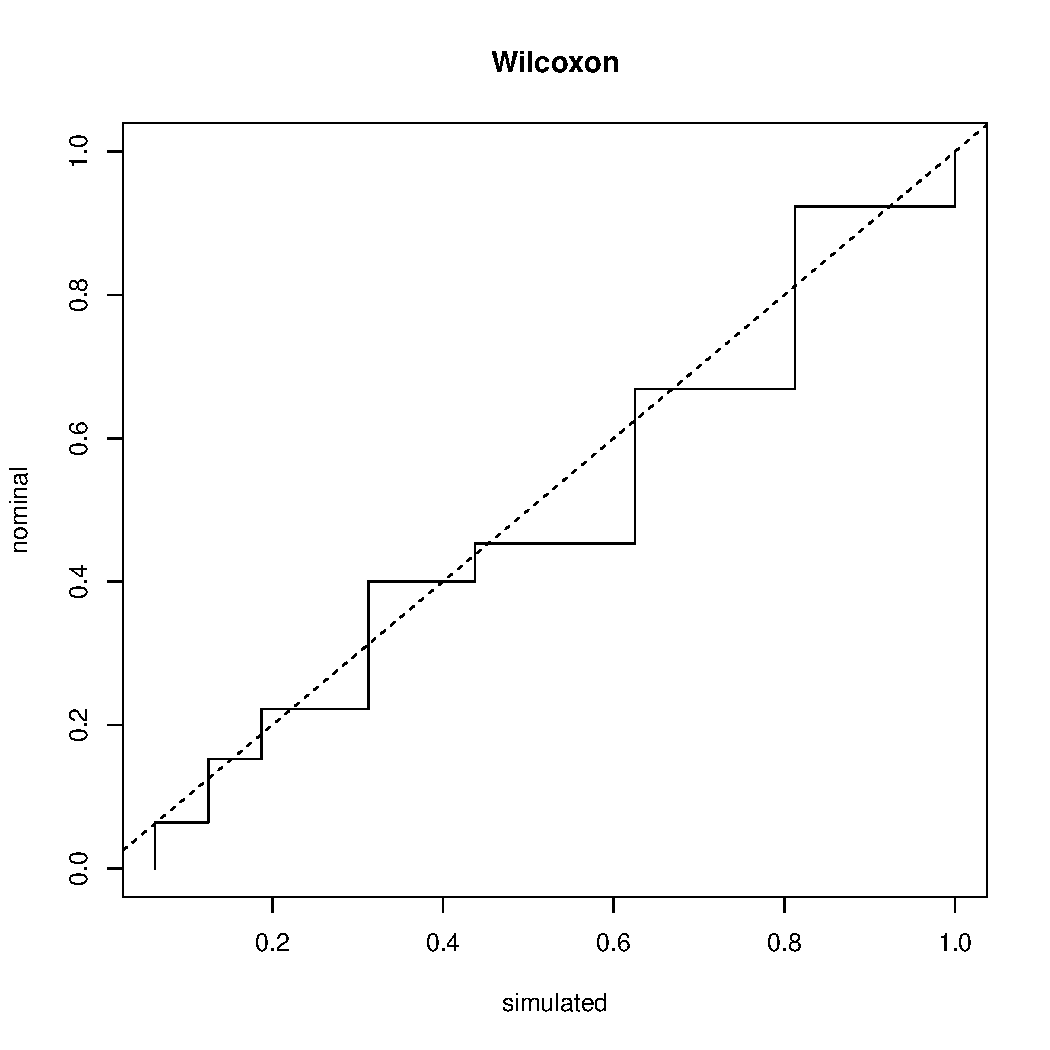
\includegraphics[width=70mm]{img/pv_weibull_05_1_n5_wilco.pdf}
 \end{center}
       \caption{$\alpha$ エラーのプロット. ワイブル分布 $\mathrm{Weibull}(0.5,1)$. $n=5$. Wilcoxon の符号付き順位検定.}
  \label{fig_pv_weibull_05_1_5_wilco}
\end{figure}

t 検定がガタガタになった. Wilcoxon の符号付き順位検定も崩れはじめた.

サンプルサイズを増やして $n=10$ のときを図\ref{fig_pv_weibull_2_1_10_t}-\ref{fig_pv_weibull_2_1_10_wilco}に示す. 

\begin{figure}[htbp]
  \begin{center}
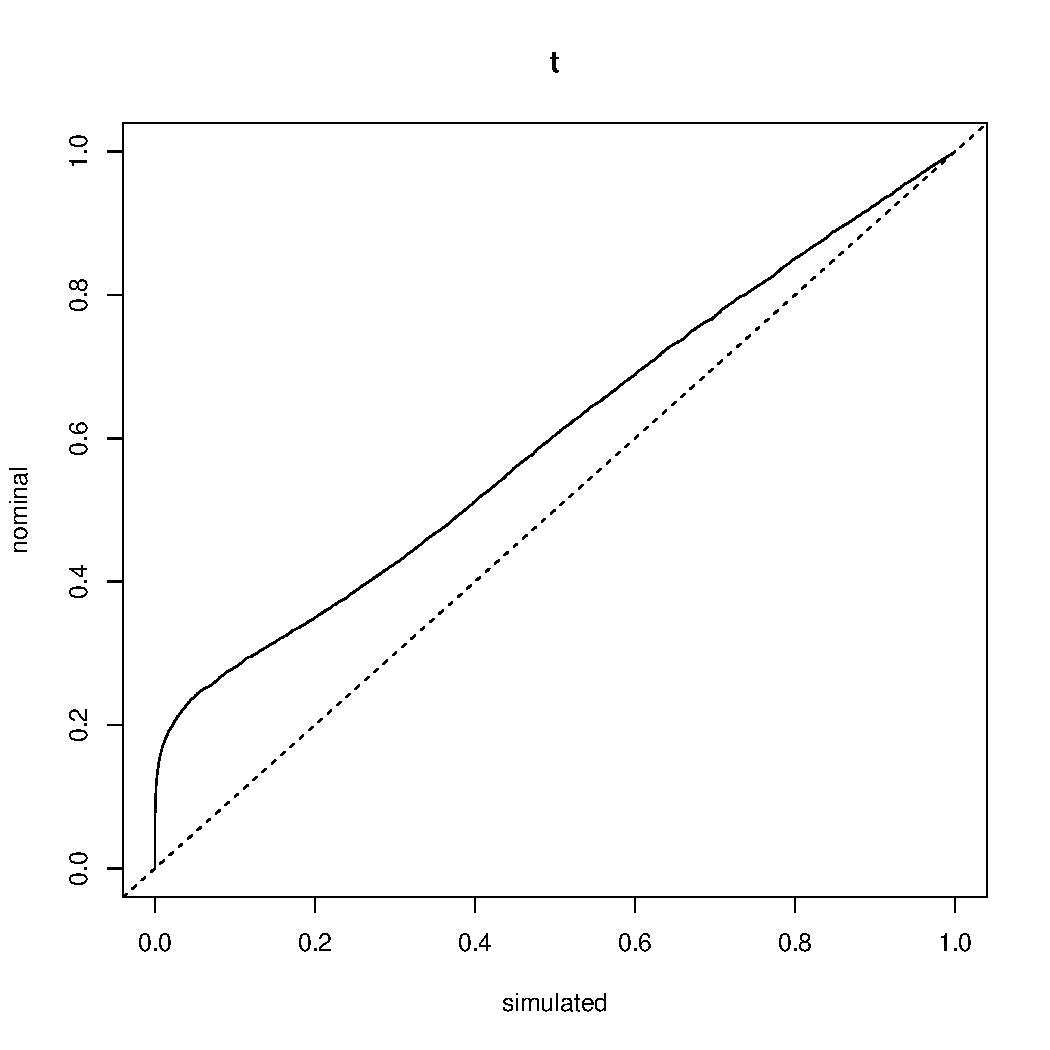
\includegraphics[width=70mm]{img/pv_weibull_05_1_n10_t.pdf}
  \end{center}
     \caption{$\alpha$ エラーのプロット. ワイブル分布 $\mathrm{Weibull}(0.5,1)$. $n=10$. t 検定}
  \label{fig_pv_weibull_05_1_10_t}
 \end{figure}
 
 \begin{figure}[htbp]
 \begin{center}
  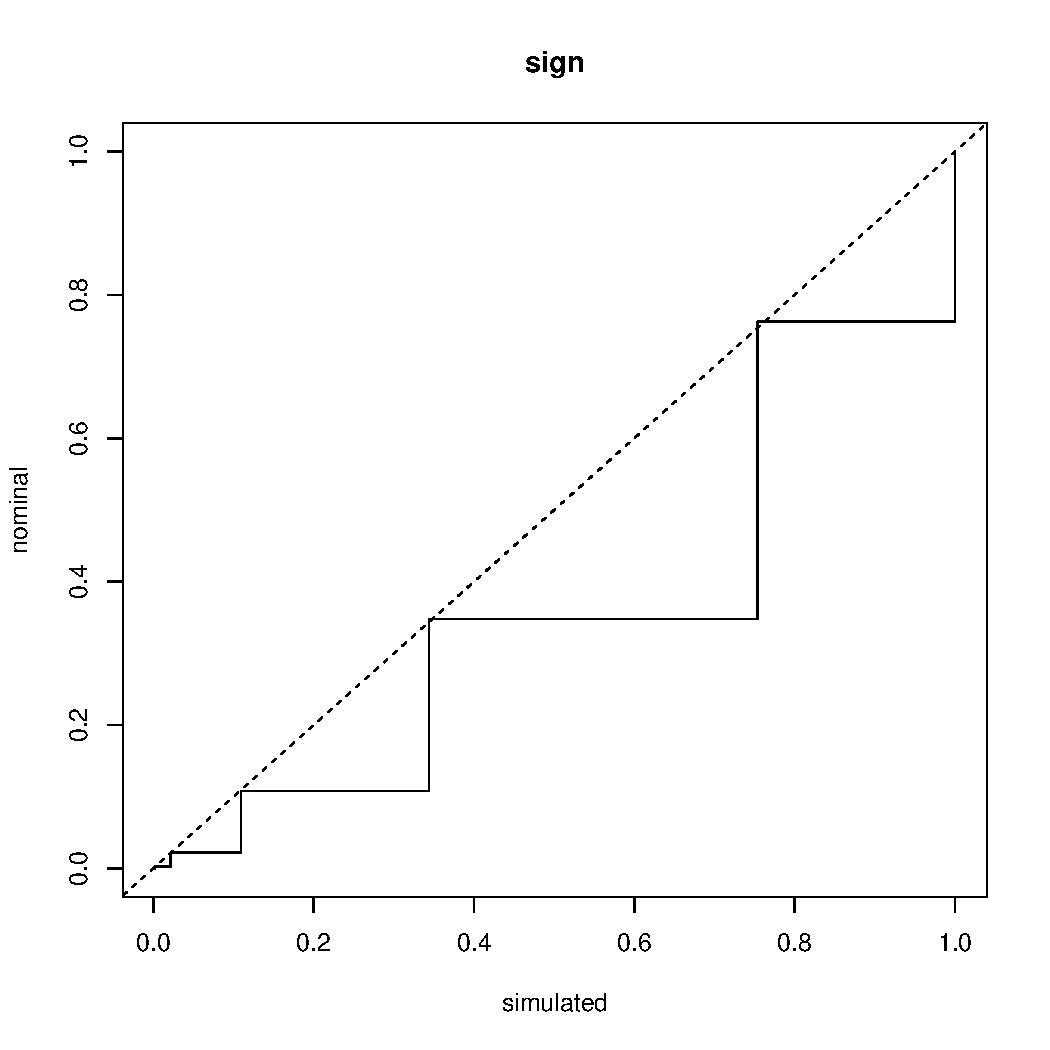
\includegraphics[width=70mm]{img/pv_weibull_05_1_n10_sign.pdf}
 \end{center}
      \caption{$\alpha$ エラーのプロット. ワイブル分布 $\mathrm{Weibull}(0.5,1)$. $n=10$. 符号検定.}
     \end{figure}  

 \begin{figure}[htbp]
 \begin{center}
  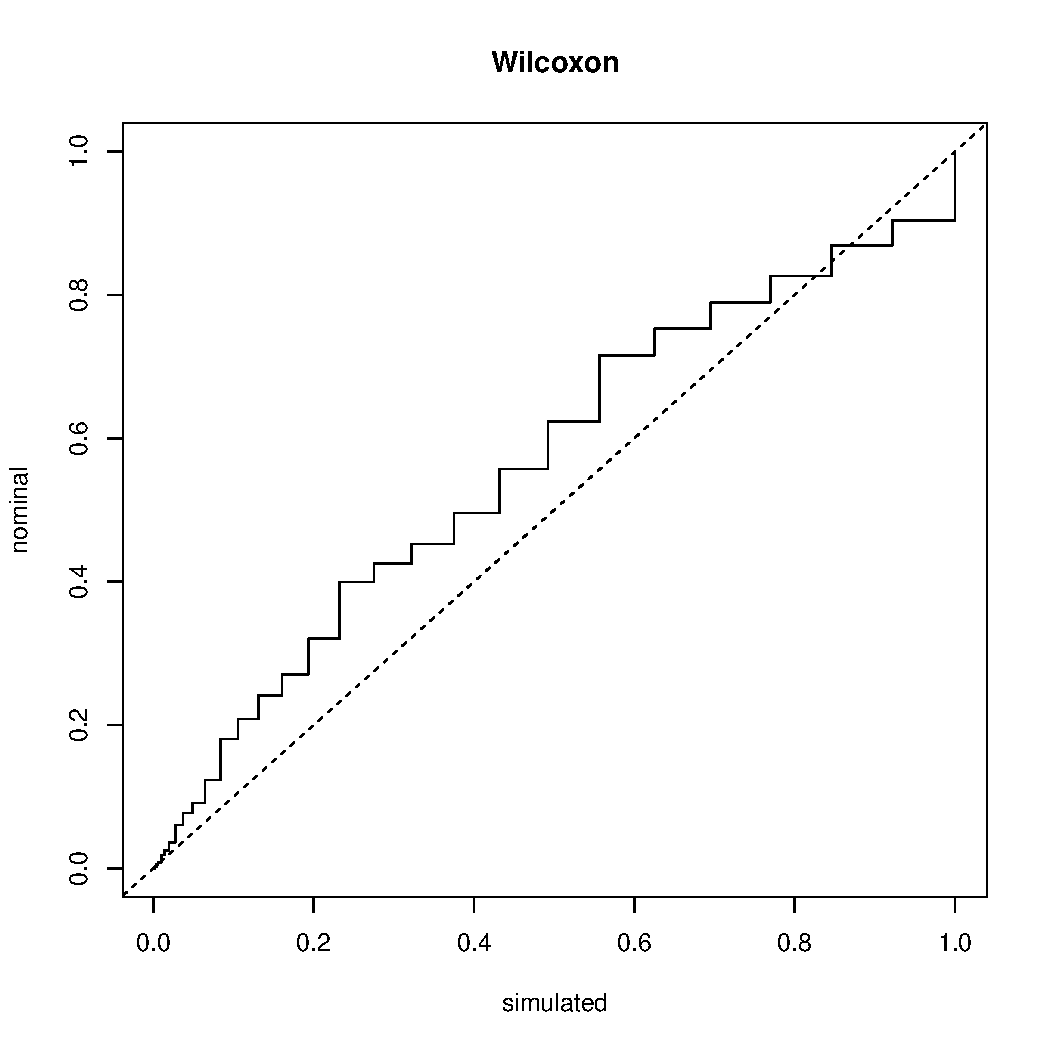
\includegraphics[width=70mm]{img/pv_weibull_05_1_n10_wilco.pdf}
 \end{center}
       \caption{$\alpha$ エラーのプロット. ワイブル分布 $\mathrm{Weibull}(0.5,1)$. $n=10$. Wilcoxon の符号付き順位検定.}
  \label{fig_pv_weibull_05_1_10_wilco}
\end{figure}

Wilcoxon の符号付き順位検定はサンプルサイズを増やすとむしろはっきり棄却するようになる.

もっとサンプルサイズを増やして $n=100$ のときを図\ref{fig_pv_weibull_2_1_100_t}-\ref{fig_pv_weibull_2_1_100_wilco}に示す. 

\begin{figure}[htbp]
  \begin{center}
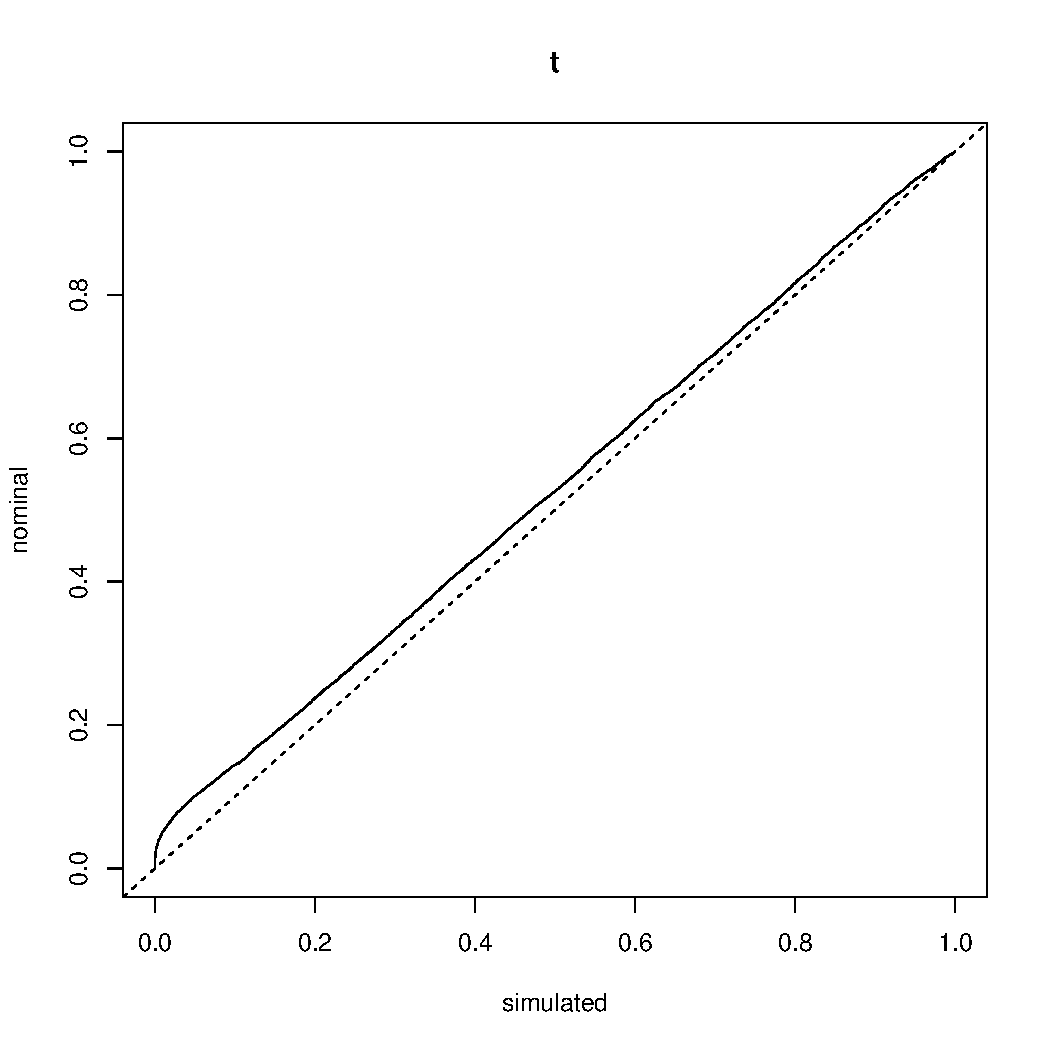
\includegraphics[width=70mm]{img/pv_weibull_05_1_n100_t.pdf}
  \end{center}
     \caption{$\alpha$ エラーのプロット. ワイブル分布 $\mathrm{Weibull}(0.5,1)$. $n=100$. t 検定}
  \label{fig_pv_weibull_05_1_100_t}
 \end{figure}
 
 \begin{figure}[htbp]
 \begin{center}
  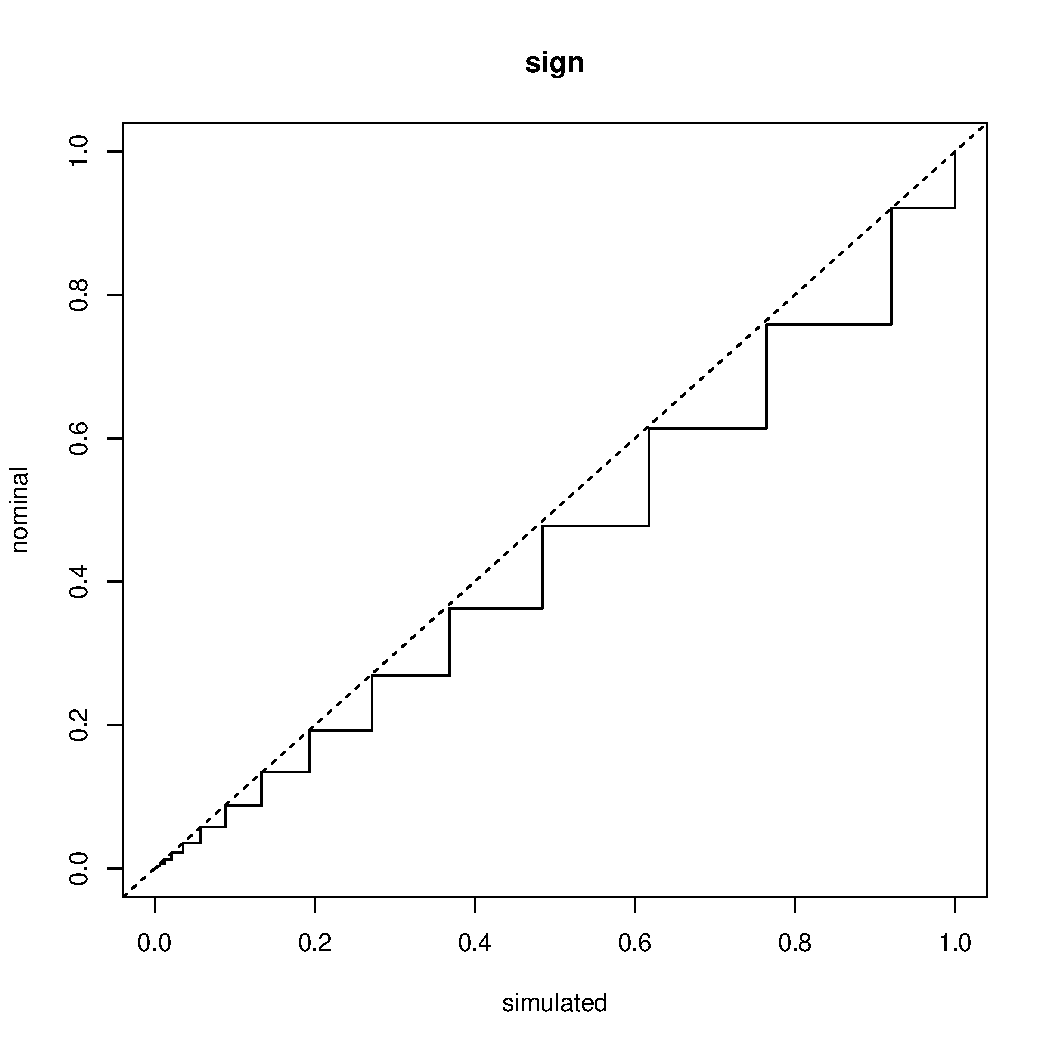
\includegraphics[width=70mm]{img/pv_weibull_05_1_n100_sign.pdf}
 \end{center}
      \caption{$\alpha$ エラーのプロット. ワイブル分布 $\mathrm{Weibull}(0.5,1)$. $n=100$. 符号検定.}
     \end{figure}  

 \begin{figure}[htbp]
 \begin{center}
  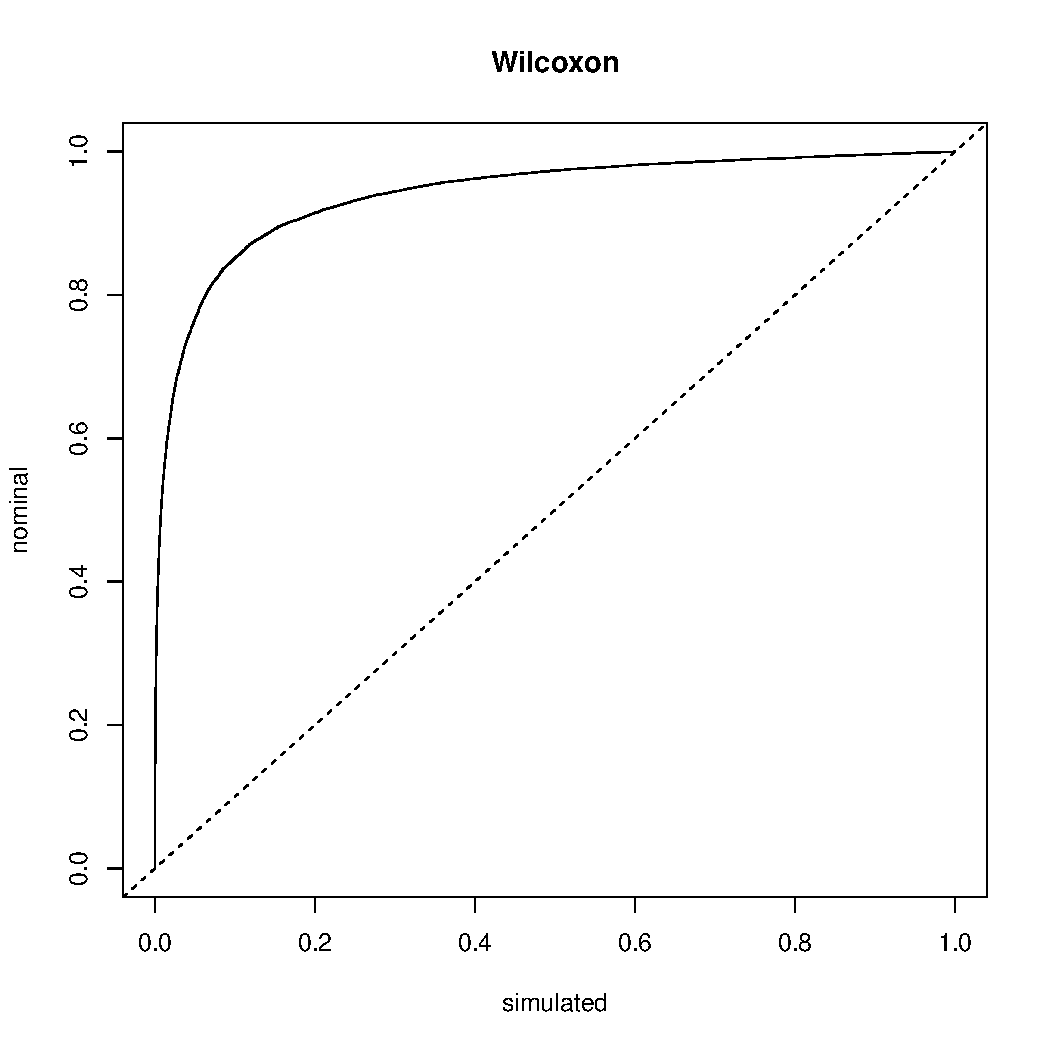
\includegraphics[width=70mm]{img/pv_weibull_05_1_n100_wilco.pdf}
 \end{center}
       \caption{$\alpha$ エラーのプロット. ワイブル分布 $\mathrm{Weibull}(0.5,1)$. $n=100$. Wilcoxon の符号付き順位検定.}
  \label{fig_pv_weibull_05_1_100_wilco}
\end{figure}

やはり Wilcoxon の符号付き順位検定はサンプルサイズを増やすとむしろはっきり棄却するようになる.

これはWilcoxon の符号付き順位検定が分布が左右対称であるという仮定を棄却していると解釈できる.

\paragraph{シミュレーションのまとめ.} 平均値や中央値に対して検定をやりたいとして, 分布の裾が明らかに重いときは, いまのところは符号検定をやるしかない. 

Wilcoxon の符号付き順位検定は, 分布が左右対称でないときは適さない. 

分布が左右対称に近いときは t 検定で概ね間に合う. 

多くの人がノンパラメトリックの検定をやりたがるのは分布が左右対称でないときだと思う.

しかし, そういう場合にWilcoxon の符号付き順位検定が教えてくれるのは, 分布が左右対称でないという事実であり, 中央値について判断するのには適さない.

 Wilcoxon の符号付き順位検定は正直, 使い所が難しいと思う.
 
 シミュレーションに用いたコードは, R フォルダにある SignTestsim.R である.
 
 \section{2群の比較}
 後で書く.
\end{document}  